\section{Elaboration Time Hardware Construction}
The methods for constructing hardware in the previous sections are all
similar in that the user directly interfaces with them. The user
directly constructs the directed subgraph of {\tt Nodes} that
implements the desired circuit and connects that subgraph to the main
graph. We refer to that class of hardware construction as 
{\it runtime} hardware construction since the hardware is
constructed as Scala is making a pass over user-written code. This
chapter discusses another class of hardware construction that we refer
to as {\it elaboration time} hardware construction since the
hardware is constructed during Chisel elaboration. This class of
hardware construction is useful since it is not always possible or
desirable for the user to construct the circuit as they are building
up the Chisel graph. The remainder of this chapter presents the
interface for writing elaboration time hardware construction routines
and three examples of how to use that interface.

\subsection{Elaboration Time Hardware Construction Interface}
The Chisel compiler mantains a list of functions that it invokes
during elaboration time to refine the input user graph of 
{\tt Nodes}. These functions must adhere to the interface described in
Figure~\ref{fig:transforms}. The bodies of the functions in
Figure~\ref{fig:transform1} varies from transformation to
transformation but will usually follow two phase format. The first
phase performs some analysis on the Chisel graph to collect
information, e.g. find all Reg nodes. The second phase will then use
the information from the first phase to construct a circuit and
perform some transformation on the graph, e.g. generate an enable
circuit for every Reg node and connect the circuit into the Reg node.

\begin{figure}[htb]
\centering
  \begin{subfigure}[t]{0.48\textwidth}
  \centering
  \caption{Elaboration Time Functions}
  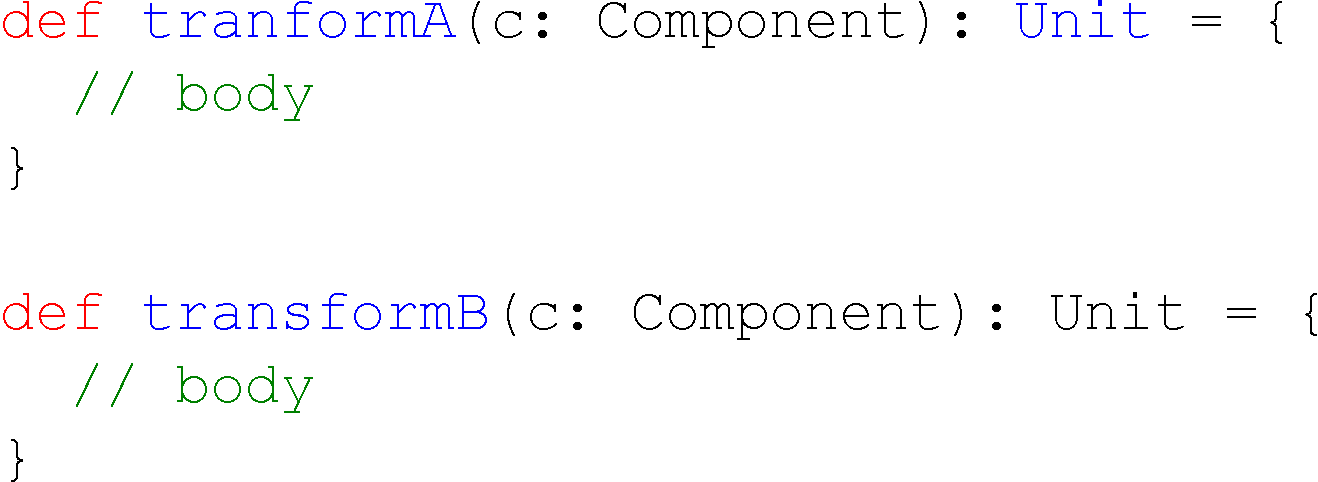
\includegraphics[width=0.9\textwidth]{figures/transform1.pdf}
  \label{fig:transform1}
  \end{subfigure}
  \hfill
  \begin{subfigure}[t]{0.48\textwidth}
  \centering
  \caption{Elaboration Time Hook}
  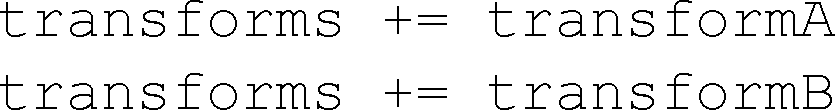
\includegraphics[width=0.7\textwidth]{figures/transform2.pdf}
  \label{fig:transform2}
  \end{subfigure}
\caption{Elaboration Time Interface}
\label{fig:transforms}
\end{figure}

\subsection{When}
Chisel provides a {\tt when - elsewhen - otherwise} statement for
performing conditional updates on {\tt Bits} and {\tt Reg}
nodes. This statement appears behaviorial but actually constructs a
hardware circuit to perform the update. The construction of this
circuit is delayed until elaboration time since it is easier to
construct the circuit once the user has specified all the updates than
it is to construct the circuit as the user is specifying
updates. 

\begin{figure}[htb]
\centering
  \begin{subfigure}[t]{0.48\textwidth}
  \centering
  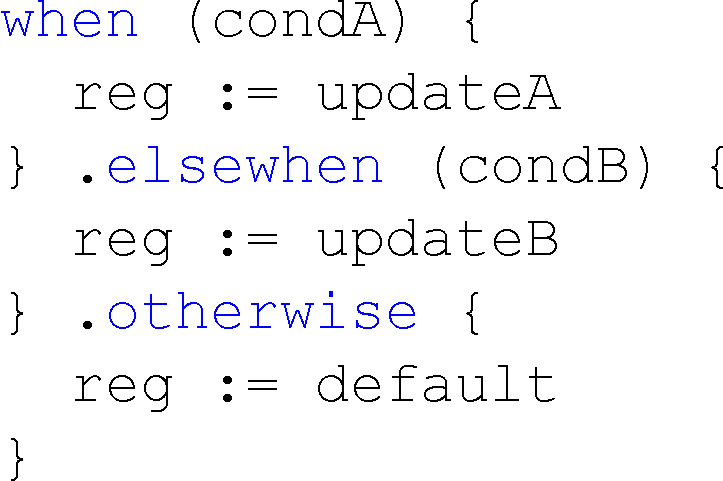
\includegraphics[width=0.7\textwidth]{figures/when.pdf}
  \caption{When Code}
  \label{fig:whenscala}
  \end{subfigure}
  \hfill
  \begin{subfigure}[t]{0.48\textwidth}
  \centering
  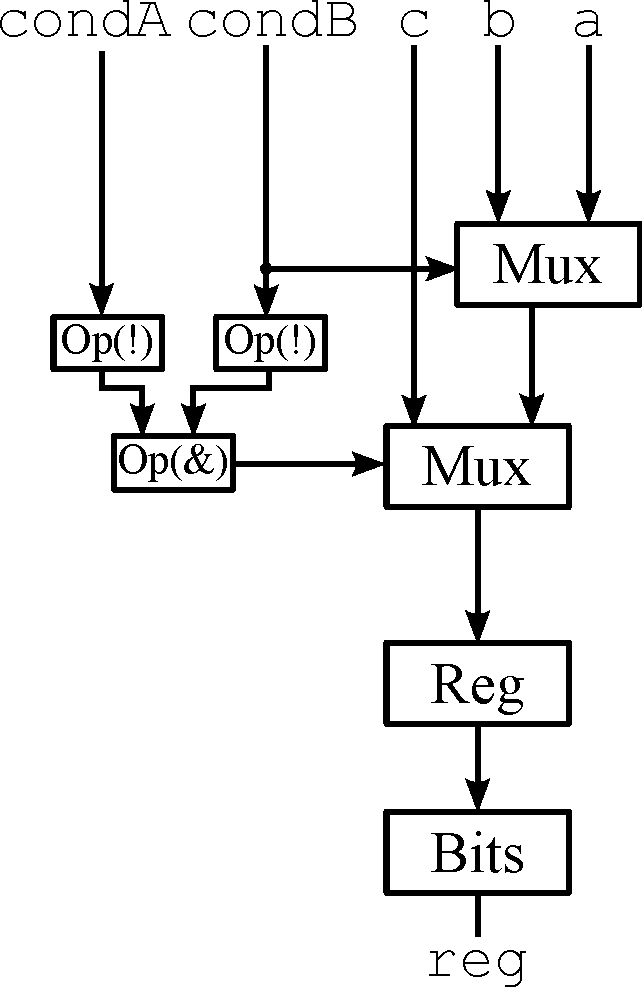
\includegraphics[width=0.5\textwidth]{figures/whengraph.pdf}
  \caption{When Graph}
  \label{fig:whenelab}
  \end{subfigure}
\caption{When Statement}
\label{fig:when}
\end{figure}

{\bf Runtime}. Instead of constructing hardware whenever a {\tt when}
statement is executed, we simply record information to be used during
elaboration. For this purpose, we maintain a mapping of node to list
of update tuples with the format {\tt (cond, bits)} where {\tt cond}
is the condition of the when statement and {\tt bits} is the update
data. These update tuples are constructed for every update statement
within the body of a {\tt when} statement and appeneded to the list
mapped to the node on the left hand side of that update
statement. Note that the updates in this list do not have to be
mutually exclusive. In the case when multiple updates are enabled,
Chisel has the semantics that the last update in program order (i.e
the last update in the list of updates) takes priority.

Figure~\ref{fig:whenscala} shows an example usage of when statements
to conditionally update a register. When this statement is executed,
it will add 3 update tuples to {\tt reg}'s list of update tuples. The
first statement adds the tuple {\tt (condA, updateA)}, the second adds
{\tt (condB \&\& !condA, updateB)}, and the third adds
{\tt (!condB \&\& !condA, updateC)}.

{\bf Elaboration Time}. The elaboration time transformation function
does not need to perform any analysis since we store all the
information for elaboration during runtime in the form of a mapping
from node to list of update tuples. For each entry in this mapping, we
construct a chain of {\tt Mux} nodes from the list of upate tuples and
connect the output of that chain into the input of the node in the
mapping. If the node in the mapping is a {\tt Reg} node then nothing
is done for the case when no updates are enabled. Otherwise, the node
in the mappng is a {\tt Bits} node and we have an additional {\tt Mux}
node to mux out a default signal provided by the user. If no default
signal is provided, Chisel reports an error to the user.

\subsection{SRAM Backend}
Users targetting the Verilog backend will want to map Mems to SRAMs
with backend specific SRAM interfaces. One way to target these SRAM
interfaces is to encode the interface into the Chisel user code. This
has the disadvantageous effect of muddling the code with SRAM specific
information and makes it an unnecesarily tedious to compile the Chisel
for a different SRAM backend.

A better way to target backend specific SRAM interfaces is to write an
elaboration time fuction that transforms the Chisel graph to target
specific SRAM interfaces. Let's say we want to target an SRAM that has
an {\tt init} pin which needs to be wired to the top level module. We
first perform either a breadth first search or depth first search to
find all {\tt Mem} nodes in the graph. For every {\tt Mem} node, we
create a new {\tt Bits} node to stand in for the {\tt init} pin. We
add this node to the {\tt Mem} node's input. Finally, we walk up the
{\tt Component} hierarchy starting at the {\tt Component} that
contains the {\tt Mem} node and ending at the top level
{\tt Component}. For every {\tt Component} along this path, we create
a new port to connect up the {\tt init} pin.

Targetting SRAM interfaces in this way allows us to decouple of the
SRAM backend from the user code. If we want to switch to a different
SRAM target we only need to switch to a different elaboration time
function and do not need to modify the user code.

\subsection{Automatic Pipeline Synthesis}
Pipelining is a commonly used microarchitectural technique for
improving the performance of a datapath. Hardware designers usually
determine upfront the desired pipeline depth and then bake the
corresponding pipelining logic into their datapath code. This approach
clutters an otherwise easily readible datapath with extraneous logic
unrelated to original functionality of the datapath, making it
difficult to modify the datapath or even change the pipeline depth. A
better approach that overcomes these issues is to move the pipelining
logic into elaboration time functions.

{\bf Pipeline Specification}. In a hand coded pipeline, the pipeline
depth and the placement of pipeline registers are baked into the
Chisel datapath code. Our approach provides the functions 
{\tt setNumStages} for specifying the pipeline depth, 
{\tt setPipelineComponent} for specifying the datapath to pipeline,
and {\tt addToPipeline } for specifying in what pipeline stage a {\tt Node}
or {\tt Component} belongs. These functions allow the user to
succinctly describe a pipeline and unclutters the datapath code since
these functions can be maintained independent of the datapath.

{\bf Pipeline Generation}. The pipeline specification functions record
information that is read during elaboration time to add pipeline
registers to the directed graph of {\tt Nodes} that the Chisel datapath
code constructs.

{\bf Hazard Detection}. Inserting pipeline registers into the datapath
graph introduces pipelining hazards that are not present in the
unpipelined datapath. Here we discuss how to handle data hazards which
result from a transaction reading a state element (a {\tt Reg} node or
{\tt Mem} node) before an earlier transaction writes to that state
element. 

We first search through the datapath graph to find all state
elements. For every state element, we determine whether or not a
hazard exists on it. If there is a hazard on a state element, we add
the hazard condition into a list. For {\tt Reg} or {\tt Mem} node, a
hazard condition exists if the node belongs in a stage that precedes the
stage of its write enable or write data signal. The actual Boolean
hazard condition is {\tt wen \&\& ren} for a {\tt Reg} node and
{\tt wen \&\& ren \&\& waddr == raddr} for a {\tt Mem} node.

{\bf Hazard Resolution - Interlocks}. The easiest way to resolve
hazards is through interlocks. This hazard resolution method requires
no additional input from the user. At the stage of every state element
with a hazard condition, we trigger a stall at that stage and all
preceding stages while inserting a bubble in the following stage until
the hazard condition is no longer asserted.

{\bf Hazard Resolution - Speculation}. Some hazards can be resolved
through speculation. In a processor pipeline, for example, we can use
speculation to remove interlocks on the PC register. Users identify
speculation points.

{\bf Hazard Resolution - Bypassing}. Bypass networks can be built to
forward results from later stages to earlier stages that need the
result instead of forcing the earlier stages to stall until results
are committed. Users identify bypassing points.
